\documentclass[xcolor=pdftex,dvipsnames,table,mathserif,aspectratio=169]{beamer}
\usetheme{metropolis}
%\usetheme{Darmstadt}
%\usepackage{times}
%\usefonttheme{structurebold}

\usepackage[english]{babel}
%\usepackage[table]{xcolor}
\usepackage{pgf,pgfarrows,pgfnodes,pgfautomata,pgfheaps}
\usepackage{amsmath,amssymb,setspace,outline}
\usepackage[latin1]{inputenc}
\usepackage[T1]{fontenc}
\usepackage{relsize}
\DeclareMathSizes{10}{10}{6}{6} 


\title [Single-agent dynamic optimization models]{Single-agent dynamic optimization models}
\author{C.Conlon - help from M. Shum and Paul Scott}
\institute{Grad IO }
\date{\today}
\setbeamerfont{equation}{size=\tiny}

\begin{document}
\begin{frame}
\titlepage
\end{frame}


\frame{
\frametitle{Why dynamic estimation? External validity}
\begin{itemize}
	\item<1-> Famous example: Hendel and Nevo's (2006) estimation of laundry detergent demand

	\medskip
	\item<2-> The long-run demand elasticity for laundry detergent might be zero (or very close)

	\medskip
	\item<3-> If detergent goes on sale periodically, we might see a nonzero short-run elasticity 
	(perhaps even a large one) as customers might purchase during the sales and store
	the detergent.

	\medskip
	\item<4-> Dynamic estimation typically involves estimating the primitives of decision makers' 
	objective functions. We might estimate the model using short-run variation, but once we 
	know the decision maker's objective function, we could simulate a response to long-run 
	variation.

\end{itemize}
}



\frame{
\frametitle{Why are dynamics difficult?}
\begin{itemize}
	\item The computational burden of solving dynamic problems blows up 
		as the state space gets large. With standard dynamic estimation techniques, 
		this is especially problematic, 
		for estimation may involve solving the dynamic problem many times. 
		
	\medskip
	\item Serially correlated unobservables and unobserved heterogeneity
	(easy to confuse with state dependence) 
	\medskip
	\item Modeling expectations
	\medskip	
	\item Solving for equilibria, multiplicity (dynamic games)
\end{itemize}
}


\frame{
\frametitle{Outline}
\begin{itemize}
	\item Introduction to dynamic estimation: Rust (1987)

	\medskip
	\item Conditional choice probabilities: Hotz and Miller (1993)

	\medskip
	\item Euler equation estimation: Scott (2014)

\end{itemize}
}


\begin{frame}{Single-agent dynamic optimization models}
Setup in Rust:
\begin{itemize}
\item Harold Zurcher manages a bus depot in Madison, WI
\item Each week he must decide to continue with the current engine $i_t=0$ and pay $c(x_{t})$ or overhaul the engine $i_t=1$ and pay fixed cost $RC$.
\item His goal is to minimize \alert{long run average cost} (discounted).
\item Buses are all  \alert{independent} of one another.
\end{itemize}
\end{frame}




\begin{frame}{Rust (1987)}
The agent makes a series of decisions $i_t,i_{t+1},\ldots \in \{0,1\}$.
\begin{eqnarray*}
\max_{\{i_1, i_2, i_3, \cdots, i_t, i_{t+1}, \cdots \}} E \sum^{\infty}_{t=1} \beta^{t-1} \pi (x_t)\\
\pi \left(i_{t},x_{t} \right)=
		\begin{cases}
		-c\left(x_{t} \right)  & \mbox{ if }i_{t}=0\\		
		 -c\left(0\right) -RC& \mbox{ if }i_{t}=1
		\end{cases}
\end{eqnarray*}
\begin{itemize}
\item When costs are increasing in mileage $(x_{it})$ then this is an \alert{optimal stopping problem}.
\item We know from Stokey Lucas Prescott (1989) that solutions to optimal stopping problems are characterized by \alert{critical value} or \alert{cutoff rule} which we call $x^*$.
\end{itemize}
\end{frame}

\begin{frame}{Rust (1987)}
\begin{itemize}
\item For those who took first year macro, this problem is trivial. 
\item But Rust had a different goal in mind
\begin{itemize}
\item Can we use the observed decisions of the agent to identify the primitives of $\pi(i_t,x_t)$?
\item Instead of just optimizing Bellman's equation, can we actually \alert{estimate parameters}?
\end{itemize}
\item Need to make two modifications: 
\begin{itemize}
\item Parameters for $c(x_t,\theta_1)$ and $RC$
\item Full support errors $\varepsilon_{t}$, otherwise can't justify why $i(x)=1$ and $i(x')=0$ if $x'>x$ at some point in the data.
\end{itemize}
\end{itemize}
\end{frame}

\begin{frame}{Model: Modified Payoff Function}
\begin{itemize}
	\item per-period profit function:\[
		\pi \left(i_{t},x_{t},\theta_{1}\right)=
		\begin{cases}
		-c\left(x_{t},\theta_{1}\right)+\varepsilon_{t}\left(0\right) & \mbox{ if }i_{t}=0\\		
		-\left(RC-c\left(0,\theta_{1}\right)\right)+\varepsilon_{t}\left(1\right) & \mbox{ if }i_{t}=1
		\end{cases}
		\]
	where \\
	\begin{itemize}
		\item $c\left(x_{t},\theta_{1}\right) $ -  regular maintenance costs (including expected breakdown costs),
		\item $RC$ - the net costs of replacing an engine,
		\item $\varepsilon$ - payoff shocks.
	\end{itemize}
	
	\item $x_{t}$ is the \alert{observed state variable} known to both agent and econometrician
	\item $\varepsilon$ is the \alert{unobserved state variable} known only to agent
\end{itemize}
\end{frame}




\begin{frame}
\frametitle{Model: Bellman}
\footnotesize
 Can define value function using Bellman equation:
 \begin{eqnarray*}
		V_{\theta}\left(x_{t},\varepsilon_{t}\right) &=& \max_{i} \left[ \pi \left(i,x_{t},\theta_1 \right) +
		\beta EV_{\theta}\left(x_{t},\varepsilon_{t},i \right) \right]\\
	 EV_{\theta}\left(x_{t},\varepsilon_{t},i_{t}\right) &=& \int V_{\theta}\left(x_{t+1},\varepsilon_{t+1}\right) p\left(x_{t+1}, \varepsilon_{t+1} |x_{t},\varepsilon_{t},i_{t},\theta_{2},\theta_{3}\right)
\end{eqnarray*}
It is helpful to define the \alert{choice-specific value function}:


\begin{eqnarray*}
\tilde V_{\theta} (x_t, \varepsilon_t, i_t) &=& \left \{ 
\begin{array}{lr}
\tilde u(x_t, 1;\theta_1) + \beta EV(0, \varepsilon ') + \varepsilon_{t}(1) & \text{ if } i_t = 1 \\
\tilde u(x_t , 0; \theta_1) + \beta E_{x', \varepsilon ' | x_t, \varepsilon_t, i_t} V(x', \varepsilon ')  + \varepsilon_{t}(0)  & \text{ if } i_t = 0
\end{array}
\right .\\
V_{\theta}(x_t,\varepsilon_t) &=& \max \left\{ \tilde V_{\theta} (x_t, \varepsilon_t, 1) + \varepsilon_{t}(1) ,\tilde V_{\theta} (x_t, \varepsilon_t, 0) + \varepsilon_{t}(0) \right\}
\end{eqnarray*}
\begin{itemize}
	\item $\theta_{1}$ - parameters of cost function
	\item $\theta_{2}$ - parameters of distribution of $\varepsilon$ (these will be assumed/normalized away)
	\item $\theta_{3}$ - parameters of $x$-state transition function
	\item $RC$ - replacement cost
	\item discount factor $\beta$ will be imputed (more on this later)
\end{itemize}
\end{frame}


\begin{frame}
\frametitle{Assumptions}
\begin{block}{First Order Markov}\end{block}\vspace{-0.5cm}
\begin{block}{Conditional Independence Assumption}
The transition density of the controlled process $\left\{x_{t},\varepsilon_{t}\right\}$ factors as:\[
p\left(x_{t+1},\varepsilon_{t+1}|x_{t},\varepsilon_{t},i_{t},\theta_{2},\theta_{3}\right)
= q\left(\varepsilon_{t+1}|x_{t+1},\theta_{2}\right)p\left(x_{t+1}|x_{t},i_{t},\theta_{3}\right)
\]
\end{block}

\begin{itemize}
	\item CI assumption is very powerful: it means we don't have to treat $\varepsilon_{t}$ as
	a state variable, which would be very difficult since it's unobserved.
\end{itemize}
\begin{block}{IID Type I EV Assumption}
For now we will also assume that $ q\left(\varepsilon_{t+1}|x_{t+1},\theta_{2}\right) =  q\left(\varepsilon_{t+1}\right)$ and $q$ is an IID Type I Extreme Value (logit) distribution.
\end{block}
\begin{itemize}
\item This is not required for identification but commonly employed to simplify estimation.
\item Rust assumes that mean is $0$ and variance is $\pi^2/6$.
\end{itemize}
\end{frame}



\begin{frame}{ Implications}
Given the assumptions:
\begin{eqnarray*}
V_{\theta}(x_t,\varepsilon_t) &=& \max \left\{ \tilde V_{\theta} (x_t, \varepsilon_t, 1) + \varepsilon_{t}(1) ,\tilde V_{\theta} (x_t, \varepsilon_t, 0) + \varepsilon_{t}(0) \right\}\\
Pr(i_t=1 | x_t,\varepsilon_t,\theta) &=& Pr\left(\varepsilon_{t}(1) - \varepsilon_{t}(0) \geq \tilde V_{\theta} (x_t, \varepsilon_t, 0) - \tilde V_{\theta} (x_t, \varepsilon_t, 1) \right) \\
&=& \frac {\exp[\tilde V_{\theta} (x_t, \varepsilon_t, 1)]  }{\exp[\tilde V_{\theta} (x_t, \varepsilon_t, 0)] + \exp[\tilde V_{\theta} (x_t, \varepsilon_t, 1)]} 
\end{eqnarray*}
This expression is logit-like. Recall the static logit:
\begin{eqnarray*}
Pr(i_t=1 | x_t,\varepsilon_t,\theta) &=& \frac {\exp[u_{\theta} (x_t, 1)]  }{\exp[u_{\theta} (x_t, 0)] + \exp[u_{\theta} (x_t, 1)]} 
\end{eqnarray*}
Problem:
\begin{itemize}
\item The general problem is that we can often write an observationally equivalent \alert{myopic model}
\item In general without additional (parametric) restrictions we are under identified (especially w.r.t $\beta$).
\end{itemize}
\end{frame}



\frame{
\frametitle{Theorem 1 preview}
\begin{itemize}
	\item Assumption CI has two powerful implications:
	\begin{itemize}
		\medskip
		\item We can write $ EV_{\theta}\left(x_{t},i_{t}\right)$ instead of $EV_{\theta}\left(x_{t},\varepsilon_{t},i_{t}\right)$,
		\medskip
		\item We can consider a Bellman equation for $ V_{\theta}\left(x_{t}\right)$, which is computationally simpler than
		the Bellman equation for $V_{\theta}\left(x_{t},\varepsilon_{t}\right) $.

	\end{itemize}
\end{itemize}
}

\frame{
\frametitle{Theorem 1}

\begin{block}{Theorem 1}
Given CI, \[
	P\left(i|x,\theta\right) = \frac{\partial}{\partial \pi \left(x,i,\theta_{1}\right)} W\left( \pi \left(x,\theta_{1}\right) +\beta EV_{\theta}\left(x\right) |x,\theta_{2}\right)
\]
and  $EV_{\theta}$ is the unique fixed point of the contraction mapping: \[
	EV_{\theta}\left(x,i\right) = \int_{y} W\left(\pi \left(y,\theta_{1}\right)+
	\beta EV_{\theta}\left(y\right)|y,\theta_{2}\right)
	p\left(dy|x,i,\theta_{3}\right)
\]
where
\begin{itemize}
	\item $P\left(i|x,\theta\right)$ is the probability of action $i$ conditional on state $x$
	\item $W\left( \cdot |x,\theta_{2}\right)$ is the surplus function: \[
	W\left(v |x,\theta_{2}\right) \equiv \int_{\varepsilon}  \max_{i} \left[v\left( i \right) +\varepsilon\left( i \right)\right] 
	q\left(d\varepsilon|x,\theta_{2}\right)	
	\]
\end{itemize}
\end{block}

}


\frame{
\frametitle{Theorem 1 example: logit shocks}
\begin{itemize}
{\small
	\item $v_{\theta}\left(x,i\right) \equiv \pi \left(x,i,\theta_{1}\right)+\beta EV_{\theta}\left(x,i\right)$ -- the \emph{conditional value function}.

	\smallskip
	\item Suppose that $\varepsilon\left(i\right)$ is distributed independenly
	across $i$ with $Pr\left(\varepsilon\left(i\right)\le\varepsilon_{0}\right)=e^{-e^{-\varepsilon_{0}}}$ -- logit shocks.
	Then,
	\[
	\begin{array}{ccl}
	W\left(v\left(x\right)\right) & = & 
	\int\max_{i}\left[v\left(x,i\right)+\varepsilon\left(i\right)\right]
	\prod_{i}e^{-\varepsilon\left(i\right)}e^{-e^{-\varepsilon\left(i\right)}}d\varepsilon\\
	\\
	 & = & \ln\left(\sum_{i}\exp\left(v\left(x,i\right)\right)\right)+\gamma
	\end{array}
	\]
	where $\gamma\approx .577216$ is Euler's gamma.

	\smallskip
	\item It is then easy to derive expressions for conditional choice probabilities:\[
	P\left(i|x,\theta\right)= \frac{\exp\left(v_{\theta}\left(x,i\right)\right)}{\sum_{i'}\exp\left(v_{\theta}\left(x,i'\right)\right)}
	\]
	\smallskip
	\item The conditional value function plays the same role as a static utility function
	when computing choice probabilities.
}
\end{itemize}
}


\begin{frame}{Rust (1987)}
Likelihood function for a single bus:
\begin{equation*}
\begin{split}
& l (x_1, \cdots , x_T, i_t, \cdots , i_T | x_0, i_0 ; \theta) \\
= & \prod^T_{t=1} Prob (i_t, x_t | x_0, i_0, \cdots , x_{t-1}, i_{t-1} ; \theta) \\
= & \prod^T_{t=1} Prob (i_t, x_t |  x_{t-1}, i_{t-1} ; \theta) \\
= & \prod^T_{t=1} Prob (i_t | x_t; \theta) \cdot \prod^T_{t=1} Prob (x_t | x_{t-1}, i_{t-1} ; \theta_3) .
\end{split}
\end{equation*}
The third line arises from the Markovian feature of the problem, and the last equality arises due to the conditional independence assumption. 
\end{frame}

\begin{frame}{Rust (1987)}
Log likelihood is additively separable in the two components:
\begin{equation*}
\text{log } l(\theta) = \sum^T_{t=1} \text{log } Prob (i_t | x_t ; \theta_1) + \sum^T_{t=1} \text{log } Prob (x_t | x_{t-1}, i_{t-1}; \theta_3).
\end{equation*}
Give the factorization of the likelihood function above, we can estimate in two steps... \\
\vspace{3mm}
\end{frame}

\begin{frame}{Step 1: Estimate Markov TPM}
\begin{itemize}
\item Estimate $\theta_3$, the parameters of the Markov transition probabilities for mileage, conditional on non-replacement of engine (i.e. $i_t = 0$)
\item Recall that $x_{t+1} = 0$ if $i_t = 1$
\end{itemize}

We assume a discrete distribution for $\triangle x_t \equiv x_{t+1} - x_t$, the incremental mileage between any two periods:
\begin{equation*}
\triangle x_t = \left \{ 
\begin{matrix}
[0, 5000) & \text{w/prob } p \\
[5000, 10000) & \text{w/prob } q \\
[10000, \infty) & \text{w/prob } 1 - p - q  
\end{matrix}
\right .
\end{equation*}
so that $\theta \equiv \{p, q \}$, with $0 < p, q< 1$ and $p + q < 1$. \\
\vspace{2mm}
\begin{itemize}
\item $\hat \theta_3$ estimated by empirical frequencies: $\hat p = \text{freq} \{ \triangle x_t \in  [0, 5000) \}$, etc. 
\item Note: this does not require the behavioral model!
\end{itemize}
\end{frame}

\begin{frame}{Step \#2: Estimate Structural Parameters of Cost Function}
Start by treating $(\beta, \hat \theta_3)$ as given:
\begin{enumerate}
\item Fix a guess of $(RC,\theta_1)$ the remaining parameters. 
\item Iterate on the Bellman Operator for $(\beta,\theta_1,\theta_3,RC)$ using \alert{Value Function Iteration} to get $V^*(x,\varepsilon)$ or $\tilde V^*(x,\varepsilon)$.
\item Calculate \alert{conditional choice probabilities} (CCPs):
\begin{eqnarray*}
Pr(i_t=1 | x_t,\varepsilon_t,\theta) &=&  \frac {\exp[ \tilde V_{\theta} (x_t, \varepsilon_t, 1)]  }{\exp[\tilde  V_{\theta} (x_t, \varepsilon_t, 0)] + \exp[ \tilde  V_{\theta} (x_t, \varepsilon_t, 1)]} 
\end{eqnarray*} 
\item Evaluate the log-likelihood:
\begin{eqnarray*}
\log l(\theta) = \sum^T_{t=1} \log \text{Pr} (i_t | x_t ; \theta_1,RC) + \underbrace{\sum^T_{t=1} \log \text{Pr} (x_t | x_{t-1}, i_{t-1}; \hat{\theta}_3)}_{\text{Can Ignore! Why?}}
\end{eqnarray*}
\end{enumerate}
Solve via MLE. This is the \alert{Nested Fixed Point} algorithm.
\end{frame}

\begin{frame}{Computational Details}
That looked easy, except that:
\begin{itemize}
\item I never really showed you how to recover $\tilde{V}_{\theta}(x,i)$.
\item Directly iterating on Bellman's operator requires keeping track of $\varepsilon$'s which are: (1) unobserved to you the econometrician and (2) continuous and full support (not a discrete grid).
\begin{itemize}
\item AKA a big pain.
\end{itemize}
\item You may (or may not) have learned some tricks for solving Bellman equations in Macro that you could apply here: VFI, Policy Iteration (PI), Howard's Policy Improvement, etc.
\begin{itemize}
\item None of that really tells us how to deal with $\varepsilon$'s.
\end{itemize}
\end{itemize}
\end{frame}

\begin{frame}{Rust's Trick}\

\begin{itemize}
\item Rust has a nice trick that let's us work with a new function $EV_{\theta}(x,i)$ instead of $V_{\theta}(x,i,\varepsilon)$ we call this the \alert{ex ante} or \alert{expected value function}.
\begin{eqnarray*}
EV(x, i) \equiv E_{x', \varepsilon ' | x, i} V(x', \varepsilon ' ; \theta)
\end{eqnarray*}
\item In words $EV_{\theta}(x,i)$ says at time $t-1$ what is the expected value of $V_{\theta}(x_t,\varepsilon_t)$ [eq 4.14].
\begin{eqnarray*}
\resizebox{.9\hsize}{!}{$EV(x,i) = \int_y \log \left \{ \sum_{j \in C(y)} \exp [ u(y,j; \theta) + \beta EV(y, j)] \right \} p(dy|x,i) $}
\end{eqnarray*}
\item Here $x, i$ denotes the \emph{previous} period's mileage and replacement choice, and $y, j$ denote the \emph{current} period's mileage and choice. 
\end{itemize}
\end{frame}

\begin{frame}{Derivation of Rust's Trick}
This \alert{ex ante value function} can be derived from Bellman's equation:
\begin{equation*}
\begin{split}
V(y, \varepsilon ;\theta) = & \max_{j \in 0,1} [ u(y, j ; \theta) + \varepsilon_j + \beta EV(y,j)] \\
\Longrightarrow & E_{y, \varepsilon} [V(y, \varepsilon ; \theta) | x, i ] \equiv  EV(x, i ; \theta) \\
= & E_{y, \varepsilon | x, i } \left \{ \max_{ j \in 0,1} [ u(y, j ; \theta) + \varepsilon_j + \beta EV(y,j)] \right \} \\
= &  E_{y | x, i }  E_{\varepsilon | x, i } \left \{ \max_{ j \in 0,1} [ u(y, j ; \theta) + \varepsilon_j + \beta EV(y,j)] \right \} \\
= &  E_{y | x, i } \log \left \{ \sum_{j=0,1} \exp [ u(y, j ; \theta)  + \beta EV(y,j)] \right \} \\
= & \int_y \log  \left \{ \sum_{j=0,1} \exp [ u(y, j ; \theta)  + \beta EV(y,j)] \right \} p(dy|x,i).
\end{split}
\end{equation*}
\end{frame}
%
%\begin{frame}{Rust (1987)}
%The next-to-last equality uses the closed-form expression for the expectation of the maximum, for extreme-value variates.\\
%\vspace{3mm}
%Once the $EV(x, i ;\theta)$ function is computed for $\theta$, the choice probabilities $p(i_t |x_t)$ can be constructed as
%\begin{equation*}
%\frac {\exp(u(x_t, i_t ;\theta) + \beta EV (x_t, i_t; \theta))}{\sum_{i=0,1} \exp(u(x_t, i;\theta) + \beta EV(x_t, i;\theta))}.
%\end{equation*}
%\end{frame}

\begin{frame}{Value Function Iteration}
\footnotesize
\begin{enumerate}
\item Start with an initial guess at $\tau=0$ for $EV^{\tau}_{\theta}(x,i)$. A common guess is $EV_{\theta}^{\tau}(x,i) = 0$ for all $(x,i)$
\item Iterate Bellman Operator
\begin{eqnarray*}
EV_{\theta}^{\tau+1}(x,i)= & \int_y \log  \left \{ \sum_{j=0,1} \exp [ u(y, j ; \theta)  + \beta EV^{\tau}(y,j)] \right \} p(dy|x,i).
\end{eqnarray*}
with $p(dy | x, i; \hat \theta_3)$ estimated in Step 1.
\item Compare $\epsilon(\tau) \equiv \sup_{(x,i)} | EV_{\theta}^{\tau+1}(x,i) - EV_{\theta}^{\tau}(x,i)|$ to $\epsilon^{tol}$. If $\epsilon(\tau) \leq \epsilon^{tol}$ then stop.
\end{enumerate}
See my notes on Numerical Dynamic Programming for more details.
\end{frame}



\begin{frame}{Value Function Iteration: Bounds}
\begin{itemize}
\item Suppose we set $V_0 =0$ then the value function iteration approach is just like solving the finite horizon problem by backward induction.
\item The CMT guarantees consistency at a geometric rate or \alert{linear} convergence with modulus $\beta$
\item We can derive an expression for the number of steps we need to get an $\epsilon$-approximation.
\begin{eqnarray*}
T(\epsilon,\beta) = \frac{1}{| \log(\beta) | } \log \left (\frac{1}{(1-\beta)\epsilon} \right)
\end{eqnarray*}
\item This tells us that when $\beta \rightarrow 1$ that VFI gets very very slow.
\end{itemize}
\end{frame}



\begin{frame}{Estimates}
\begin{center}
\hspace*{-.5cm}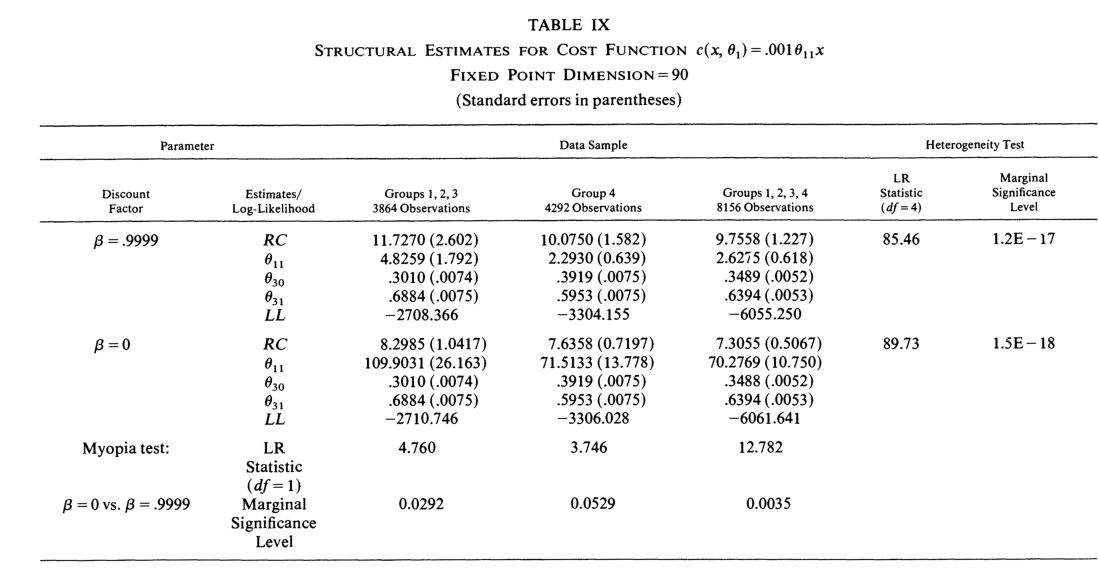
\includegraphics[scale=.65]{./resources/RustT9.pdf}
\end{center}
\end{frame}

\begin{frame}{Discount factor}
\begin{itemize}
	\item While Rust finds a better fit for $\beta=.9999$ than $\beta=0$, he finds that high levels
	of $\beta$ basically lead to the same level of the likelihood function.

	\medskip
	\item Furthermore, the discount factor is non-parametrically non-identified. Note:
	He loses ability to reject $\beta=0$ for more flexible cost function specifications.

\end{itemize}
\end{frame}


\begin{frame}{Discount factor}
\begin{center}
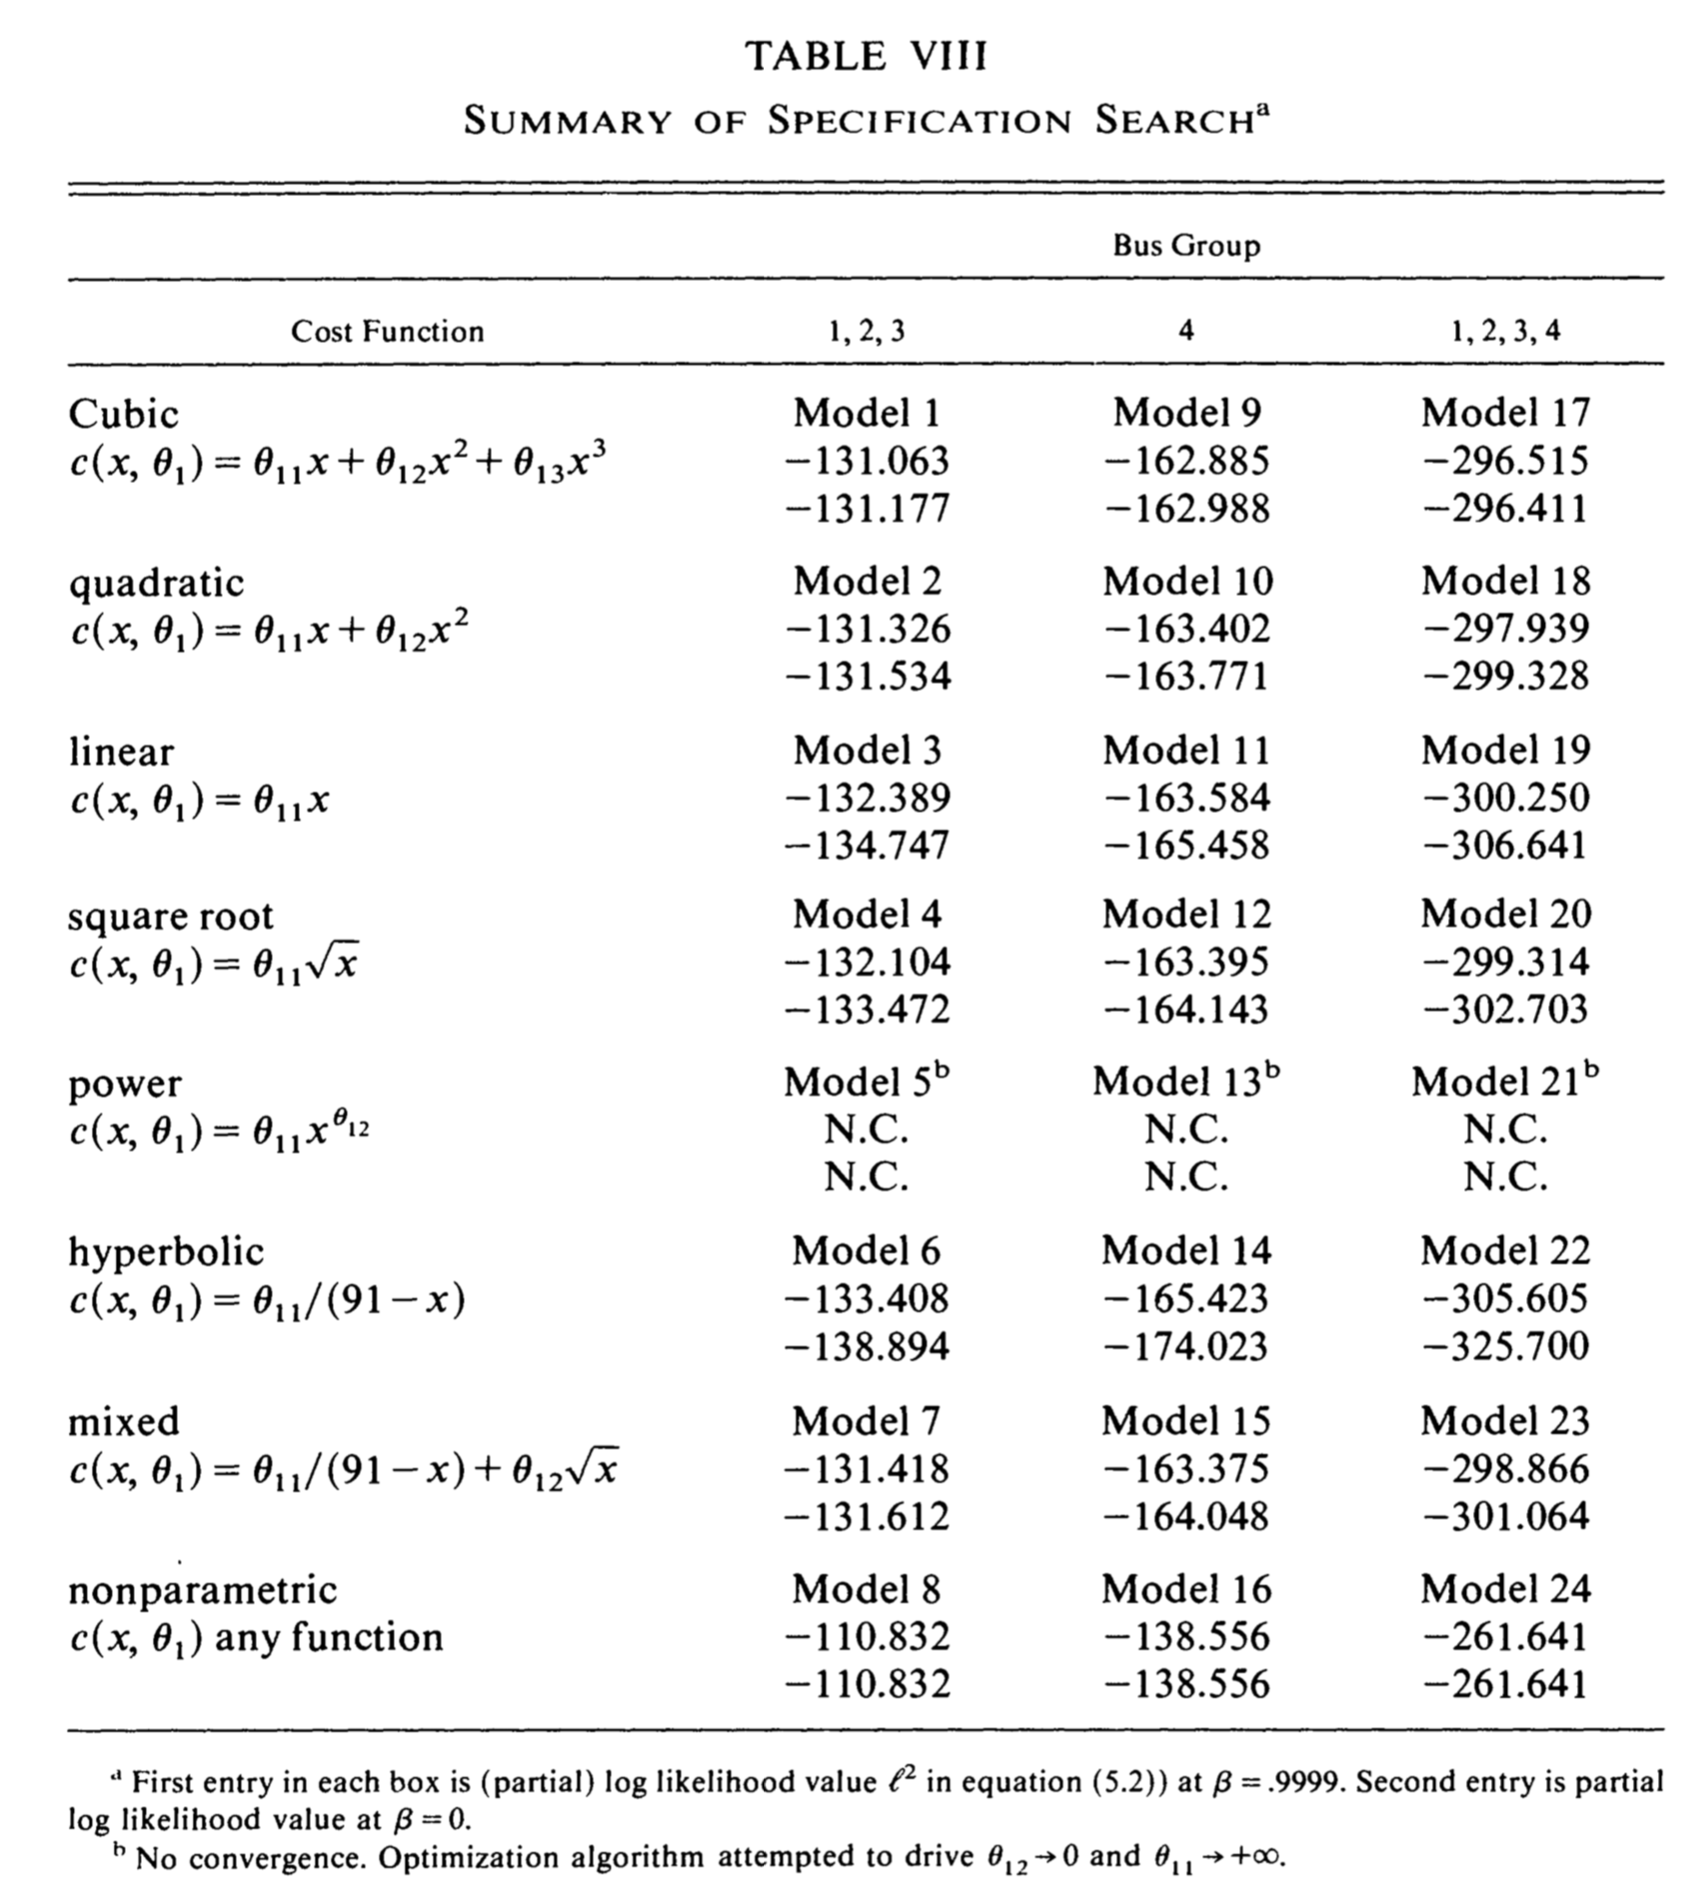
\includegraphics[scale=.25]{./resources/RustT8.png}
\end{center}
\end{frame}

\begin{frame}{Application}
\begin{center}
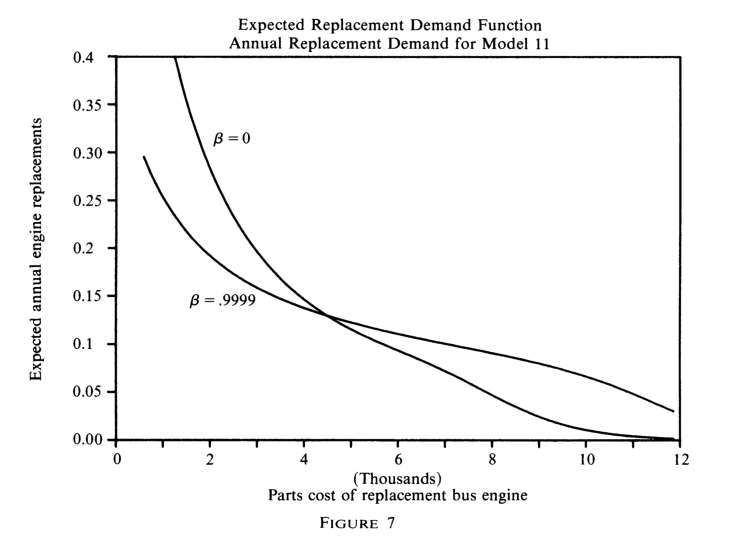
\includegraphics[scale=.8]{./resources/RustF7.pdf}
\end{center}
\end{frame}

\begin{frame}{MPEC}
\begin{center}
Cut to MPEC Slides Here
\end{center}
\end{frame}


%
%\begin{frame}
%\frametitle{Generalization of Rust: Theorem 1}
%
%\begin{block}{Theorem 1}
%Given CI, \[
%	P\left(i|x,\theta\right) = \frac{\partial}{\partial \pi \left(x,i,\theta_{1}\right)} W\left( \pi \left(x,\theta_{1}\right) +\beta EV_{\theta}\left(x\right) |x,\theta_{2}\right)
%\]
%and  $EV_{\theta}$ is the unique fixed point of the contraction mapping: \[
%	EV_{\theta}\left(x,i\right) = \int_{y} W\left(\pi \left(y,\theta_{1}\right)+
%	\beta EV_{\theta}\left(y\right)|y,\theta_{2}\right)
%	p\left(dy|x,i,\theta_{3}\right)
%\]
%where
%\begin{itemize}
%	\item $P\left(i|x,\theta\right)$ is the probability of action $i$ conditional on state $x$
%	\item $W\left( \cdot |x,\theta_{2}\right)$ is the surplus function: \[
%	W\left(v |x,\theta_{2}\right) \equiv \int_{\varepsilon}  \max_{i} \left[v\left( i \right) +\varepsilon\left( i \right)\right] 
%	q\left(d\varepsilon|x,\theta_{2}\right)	
%	\]
%\end{itemize}
%\end{block}
%\end{frame}
%
%\begin{frame}
%\frametitle{Theorem 1 example: logit shocks}
%\begin{itemize}
%{\small
%	\item $v_{\theta}\left(x,i\right) \equiv \pi \left(x,i,\theta_{1}\right)+\beta EV_{\theta}\left(x,i\right)$ -- the \emph{conditional value function}.
%
%	\smallskip
%	\item Suppose that $\varepsilon\left(i\right)$ is distributed independenly
%	across $i$ with $Pr\left(\varepsilon\left(i\right)\le\varepsilon_{0}\right)=e^{-e^{-\varepsilon_{0}}}$ -- logit shocks.
%	Then,
%	\[
%	\begin{array}{ccl}
%	W\left(v\left(x\right)\right) & = & 
%	\int\max_{i}\left[v\left(x,i\right)+\varepsilon\left(i\right)\right]
%	\prod_{i}e^{-\varepsilon\left(i\right)}e^{-e^{-\varepsilon\left(i\right)}}d\varepsilon\\
%	\\
%	 & = & \ln\left(\sum_{i}\exp\left(v\left(x,i\right)\right)\right)+\gamma
%	\end{array}
%	\]
%	where $\gamma\approx .577216$ is Euler's gamma.
%
%	\smallskip
%	\item It is then easy to derive expressions for CCPs:\[
%	P\left(i|x,\theta\right)= \frac{\exp\left(v_{\theta}\left(x,i\right)\right)}{\sum_{i'}\exp\left(v_{\theta}\left(x,i'\right)\right)}
%	\]
%	\smallskip
%	\item The conditional value function plays the same role as a static utility function
%	when computing choice probabilities.
%}
%\end{itemize}
%\end{frame}

\section{CCPs and Sufficient Statistics: Hotz-Miller (1993)}


\begin{frame}{Motivation}
\begin{itemize}
	\item In Rust, we started with a guess of parameters $\theta$, iterated on the Bellman operator to get $EV_{\theta}(x,i)$ and then constructed CCP's $P(i | x, \theta)$.
	\item A disadvantage of Rust's approach is that it can be computationally intensive
	\begin{itemize}
	
		\item With a richer state space, solving value function (inner fixed point) 
		can take a very long time,
		which means estimation will take a very, very long time.
	\end{itemize}
	\item Hotz and Miller's idea is to use observable data to form an estimate 
	of (differences in) the value function from conditional choice probabilities (CCP's)
\begin{itemize}
\item We observe $P(i | x)$ directly in the data!
\end{itemize}
	
	\item The central challenge of dynamic estimation is computing continuation values. 
	In Rust, they are computed by solving the dynamic problem.
	With Hotz-Miller (or the CCP approach more broadly), we ``measure'' continuation
	values using a function of CCP's.
	
\end{itemize}
\end{frame}

\begin{frame}
\frametitle{Rust's Theorem 1: Values to CCP's}
\begin{itemize}
	\item In Rust (1987), CCPs can be derived from the value function:\[
		p_{j}\left( x\right) = \frac{\partial}{\partial \pi_{j} \left(x \right)} W\left( \pi\left( x \right) 
		+\beta E\left[V\left(x' \right)|x,j\right]\right)
	\]
	where  $W\left(u\right) = \int \max_{j} \left\{ u_{j} +\varepsilon_{j}\right\}dG\left( \varepsilon\right)$ is the surplus function.

	\medskip
	\item For the logit case:\[
	p_{j}\left(x\right) = \frac{\exp\left(v_{j}\left(x\right)\right)}{\sum_{j'\in J}\exp\left(v_{j'}\left(x\right)\right)}
	\]
	where the choice specific value function for action $j$ in state $x$ is \[
	v_{j}\left(x\right) \equiv \pi_{j}\left(x\right)+\beta E\left[V\left(x' \right)|x,j\right]
	\]
\end{itemize}
\end{frame}


\begin{frame}
\frametitle{HM's Proposition 1: CCP's to Values}
\begin{itemize}
	\item Notice that CCP's are unchanged by subtracting some constant from every conditional (choice-specific) value function. Thus, consider\[
	D_{j,0} v\left(x\right) \equiv v_{j}\left(x\right) - v_{0}\left(x\right)
	\]
	where $0$ denotes some reference action.
	
	\medskip
	\item Let $Q:\, \mathbb{R}^{\left| \mathbf{I}\right|-1} \rightarrow \Delta^{\left| \mathbf{I}\right|}$ be the mapping
	from the differences in conditional (choice-specific) values to CCP's.

	\medskip
	\item Note: we're taking for granted that the distribution of $\varepsilon$ is identical across states, otherwise
	$Q$ would be different for different $x$.

	\begin{block}{Hotz-Miller Inversion}
	$Q$ is invertible.
	\end{block}

\end{itemize}
\end{frame}

\begin{frame}
\frametitle{HM inversion with logit errors}
\begin{itemize}
	\item Again, let's consider the case of where $\varepsilon$ is i.i.d type I EV.

	\smallskip
	\item Expression for CCP's: \[
	p_{j}\left(x\right) = \frac{\exp\left(v_{j}\left(x\right)\right)}{\sum_{j'\in \mathbf{J}}\exp\left(v_{j}\left(x\right)\right)}.
	\]

	\smallskip
	\item The HM inversion follows by taking logs and differencing across actions: \[
		\ln p_{j}\left(x\right) - \ln p_{0}\left(x\right) = v_{j}\left(x\right) - v_{0}\left(x\right)
	\]

	\smallskip
	\item Thus, in the logit case (this looks a lot like Berry (1994)):
	\[
	Q_{j}^{-1} \left( p \right) = \ln p_{j} - \ln p_{0}
	\]

	\smallskip
	\item From now on, I will use $\phi(p)$ to denote $Q^{-1}(p)$.

\end{itemize}
\end{frame}


\begin{frame}{Arcidiacono and Miller's Lemma}

An equivalent result to the HM inversion was introduced by Arcidiacono and Miller (2011). 
It's worth introducing here because it makes everything from now on much simpler
and more elegant.


\begin{block}{Arcidiacono Miller Lemma}
For any action-state pair $\left(a,x\right)$, there exists a function
$\psi$ such that 
\begin{eqnarray*}
V\left(x\right)=v_{a}\left(x\right)+\psi_{a}\left(p\left(x\right)\right)
\end{eqnarray*}
\end{block}

Proof:
\begin{eqnarray*}
\begin{array}{ccl}
V\left(x\right) & = & \int\max_{j}\left\{ v_{j}\left(x\right)+\varepsilon_{j}\right\} dG\left(\varepsilon_{j}\right)\\
\\
 & = & \int\max_{j}\left\{ v_{j}\left(x\right)-v_{a}\left(x\right)+\varepsilon_{j}\right\} dG\left(\varepsilon_{j}\right)-v_{a}\left(x\right)\\
\\
 &  & \int\max_{j}\left\{ \phi_{ja}\left(p\left(x\right)\right)+\varepsilon_{j}\right\} dG\left(\varepsilon_{j}\right)-v_{a}\left(x\right)
\end{array}
\end{eqnarray*}
Letting $\psi_{a}\left(p\left(x\right)\right)=\int\max_{j}\left\{ \phi_{ja}\left(p\left(x\right)\right)+\varepsilon_{j}\right\} dG\left(\varepsilon_{j}\right)$ completes the proof
\end{frame}


\begin{frame}
\frametitle{Important relationships}
\begin{itemize}
\item The Hotz-Miller Inversion allows us to map from CCP's to differences
in conditional (choice-specific) value functions:
\begin{eqnarray*}
\phi_{ja}\left(p\left(x\right)\right)=v_{j}\left(x\right)-v_{a}\left(x\right)
\end{eqnarray*}
\medskip
\item The Arcidiacono and Miller Lemma allows us to relate ex ante and conditional (choice specific)
value functions: 
\begin{eqnarray*}
V\left(x\right)=v_{j}\left(x\right)+\psi_{j}\left(p\left(x\right)\right)
\end{eqnarray*}
\item For the logit case:
\begin{eqnarray*}
\begin{array}{ccl}
\phi_{ja}\left(p\left(x\right)\right) & = & \ln\left(p_{j}\left(x\right)\right)-\ln\left(p_{a}\left(x\right)\right)\\
\\
\psi_{j}\left(p\left(x\right)\right) & = & -\ln\left(p_{j}\left(x\right)\right)+\gamma
\end{array}
\end{eqnarray*}
where $\gamma$ is Euler's gamma
\end{itemize}
\end{frame}



\frame{
\frametitle{Estimation example: finite state space I}
\begin{itemize}
\item Let's suppose that $X$ is a finite state space. Furthermore, let's ``normalize'' the
	payoffs for 
	 a reference action $\pi_{0}\left(x\right)=0$ for all $x$.
	\begin{itemize}
		\item We'll discuss soon whether this should really be called a ``normalization'' 
	\end{itemize}
\medskip
	\item Using vector notation, recall the definition of the choice-specific value function
	for the reference action:\[
\begin{array}{ccl}
v_{0} & = & \pi_{0}+\beta F_{0}V\\
\\
v_{0} & = & \beta F_{0}V
\end{array}
\]
\medskip
	\item Using the Arcidiacono-Miller Lemma,\[
\begin{array}{ccl}
V-\psi_{0}\left(p\right) & = & \beta F_{0}V\\
 & \Rightarrow\\
V & = & \left(I-\beta F_{0}\right)^{-1}\psi_{0}\left(p\right)
\end{array}
\]

\end{itemize}
}

\frame{
\frametitle{Estimation example: finite state space II}
\begin{itemize}
	\item Now we have an expression for the ex ante value function
	that only depends on objects we can estimate in a first stage: \[
V  =  \left(I-\beta F_{0}\right)^{-1}\psi_{0}\left(p\right)
	\]

	\item To estimate the utility function for the other actions, \[
\begin{array}{ccl}
v_{j} & = & \pi_{j}+\beta F_{j}V\\
\\
V-\psi_{j}\left(p\right) & = & \pi_{j}+\beta F_{j}V\\
\\
\pi_{j} & = & -\psi_{j}\left(p\right)+\left(I-\beta F_{j}\right)V\\
\\
\pi_{j} & = & -\psi_{j}\left(p\right)+\left(I-\beta F_{j}\right)\left(I-\beta F_{0}\right)^{-1}\psi_{0}\left(p\right)
\end{array}
\]
\end{itemize}
}


\frame{
\frametitle{Identification of Models I}
\begin{itemize}
	\item If we  run through the above argument with $\pi_{0}$ fixed to 
	an arbitrary vector $\widetilde{\pi}_{0}$ rather than 0, we will arrive at the
	following:\[
		\pi_{j} = A_{a} \widetilde{\pi}_{0} + b_{j} 
	\]
	where $ A_{a} $ and $b_{a} $ depend only on things we can estimate in a first
	stage: \[
	\begin{array}{ccc}
	A_{j} & = & \left(1-\beta F_{j}\right)\left(1-\beta F_{0}\right)^{-1}\\
	\\
	b_{j} & = & A_{j}\psi_{0}\left(p\right)-\psi_{j}\left(p\right)
	\end{array}
	\]

	\smallskip
	\item We can plug in any value for $\widetilde{\pi}_{0}$, and each value
	will lead to a different utility function (different values for $\pi_{j}$). Each
	of those utility functions will be perfectly consistent with the CCP's we observe.

\end{itemize}
}

\frame{
\frametitle{Identification of Models II}
\begin{itemize}
	\item Another way to see that the utility function is under-identified:
 If there are $\left|X\right|$ states and $\left|J\right|$ actions,
the utility function has $\left|X\right|\left|J\right|$ parameters.
However, there are only $\left|X\right|\left(\left|J\right|-1\right)$
linearly independent choice probabilities in the data, so we have
to restrict the utility function for identification. 
\medskip
\item Magnac and Thesmar (2002) make this point as part of their broader
characterization of identification of DDC models. Their main result says
that we can specify a vector of utilities for the reference action
$\widetilde{\pi}$, a distribution for the idiosycratic shocks $G$,
and a discount factor, and we will be able to find a model rationalizing
the CCPs that features $\left(\widetilde{\pi},\beta,G\right)$.

\end{itemize}
}

\begin{frame}{Identification of Counterfactuals}
\begin{itemize}
\item Note that imposing a restriction like $\forall x:\pi_{0}\left(x\right)=0$
is NOT a normalization in the traditional sense. If we were talking
about a static normalization, each $x$ would represent a different
utility function, and $\pi_{0}\left(x\right)=0$ would simply be a
level normalization. However, in a dynamic model, the payoffs in one
state affect the incentives in other states, so this is a substantive
restriction.

\medskip
\item What is less clear \emph{a priori} is whether these restrictions matter for counterfactuals.
It turns out that some (but not all!) counterfactuals ARE identified, in spite of the
under-identification of the utility function. What this means is that whatever value
$\widetilde{\pi}_{0}$ we impose for the reference action, the model will not only
rationalize the observed CCP's but also predict the same counterfactual CCP's.
Kalouptsidi, Scott, and Souza-Rodrigues (2016) sort out when counterfactuals
of DDC models are identified and when they are not.
\end{itemize}
\end{frame}

\begin{frame}{Extensions}
\begin{itemize}
\item Just like we can write the BLP (1995) problem as an \alert{MPEC}, we can do the same with Rust (1987). [See my MPEC notes].
\item We cheated a bit because we assumed that not only were actions discrete but so was the state space. This trick is often attributed to Pesendorfer and Schmidt-Dengler (ReStud 2008).
\item If the state space is not discrete we need to do some forward-simulation [next slide]. (Hotz, Miller, Sanders, Smith ReStud 1994).
\item Others have extended these ideas to \alert{dynamic games}. See Aguirragabiria and Mira (Ecma 2002/2008) and Bajari Benkard and Levin (Ecma 2007).
\item Srisuma and Linton (2009) [very hard] show how to use Friedholm integral equations of 2nd kind to extend to continuous case.
\end{itemize}
\end{frame}


\begin{frame}{From NDP Notes: Policy Iteration (Howard 1960)}
An alternative to value function iteration is policy function iteration. 
\begin{itemize}
\item Make a guess for an initial policy, call it $a(s) = \arg \max_a U(a,s)$ that maps each state into an action
\item Assume the guess is stationary compute the implied $V(a,s)$
\item Improvement Step: improve on policy $a_0$ by solving 
\begin{eqnarray*}
a' = \arg \max_a U(a,s) + \beta \sum_{s'} V(a,s') p(s' | s,a)
\end{eqnarray*}
\item Helpful to define $p(\tilde{s}' | s)$ as transition probability under optimal choice $a(s)$.
\item Determine if $\| a' -a\| < \epsilon$. If yes then we have found the optimal policy $a^* $ otherwise we need to go back to step 2.
\end{itemize}
\end{frame}

\begin{frame}{From NDP Notes:  Policy Iteration (Howard 1960)}
Policy Iteration is even easier if choices AND states are discrete.
\begin{itemize}
\item For Markov transition matrix $\sum_j P_{ij} =1$ ,we want $\pi P = \pi$
\item $\lim_{t \rightarrow \infty} P^t = \pi$ where the $j$th element of $\pi$ represents the long run probability of state $j$.
\item We want the eigenvalue for which $\lambda = 1$.
\end{itemize}
Now updating the value function is easy for $k$th iterate of PI
\begin{eqnarray*}
V^k(s) &=& Eu(a^k(s),s) + \beta \tilde{P}^k V^k(s)\\
\Rightarrow V^k(s) &=& [1 - \beta \tilde{P}^k]^{-1} Eu(a^k(s),s)
\end{eqnarray*}
\begin{itemize}
\item Very fast when $\beta > 0.95$ and $s$ is relatively small. (Rust says 500 more like 5000).
\item Inverting a large matrix is tricky
\item \alert{This trick is implicit in the HM/AM formulation}.
\end{itemize}
\end{frame}


\begin{frame}{Continuous State Space}
When state space is continuous instead of discrete:\\
Approximation to the problem:
\begin{eqnarray*}
\hat{V}(s) = \max_{a \in \hat{A}(s)} \left[ (1-\beta) u(s,a) + \beta \sum_{k=1}^N \hat{V}(s')p_N (s_k' | s,a) \right]
\end{eqnarray*}
Exact Problem
\begin{eqnarray*}
V(s) = \max_{a \in A(s)} \left[ (1-\beta) u(s,a) + \beta \int V(s')p(ds' | s,a) \right]
\end{eqnarray*}
\begin{itemize}
\item Now we need to do actual numerical integration instead of just summation.
\item We cannot use the $[I- \beta P]^{-1}$ to get the ergodic distribution.
\item Usually requires interpolating between grid points to evaluate $EV(\cdot)$.
\end{itemize}
\end{frame}


\begin{frame}{Forward Simulation}
In practice, "truncate" the infinite sum at some period $T$: 
\begin{eqnarray*} 
&& \tilde V(x, d=1;\theta) =\\
&& u(x, d=1; \theta) + \beta E_{x'|x, d=1} E_{d'|x'} E_{\epsilon''|d', x'} [u(x', d';\theta) + \epsilon' \\
&& + \beta E_{x''|x', d''} E_{d''|x''} E_{\epsilon'|d'', x''} [u(x'', d'';\theta) + \epsilon'' + \cdots \\
&& \beta E_{x^T|x^{T-1}, d^{T-1}} E_{d^T|x^T} E_{\epsilon^T|d^T, x^T} [u(x^T, d^T;\theta) + \epsilon^T ]]]
\end{eqnarray*}
Also, the expectation $E_{\epsilon|d, x}$ denotes the expectation of the $\epsilon$ conditional choice $d$ being taken, and current mileage $x$. For the logit case, there is a closed form:
$$ E[\epsilon | d, x] = \gamma - \log(PR(d|x))$$
where $\gamma$ is Euler's constant ($0.577\cdots$) and $Pr(d|x)$ is the choice probability of action $d$ at state $x$. \\
\vspace{2mm}
Both of the other expectations in the above expressions are observed directly from the data. 
\end{frame}

\begin{frame}{Forward Simulation}
Choice-specific value functions can be simulated by (for $d=1,2$): 
\begin{eqnarray*}
\tilde V (x, d; \theta) \approx = & \frac 1 S \sum_s [ u(x, d;\theta) + \beta [ u(x'^s, d'^s;\theta) + \gamma - \log(\hat P(d'^s|x'^s)) \\
& +\beta [ u(x''^s, d''^s;\theta) + \gamma - \log (\hat P (d''^s |x''^s)) + \beta \cdots ]]]
\end{eqnarray*}
where:
\begin{itemize}
\item $x'^s \sim \hat G(\cdot | x, d)$ 
\item $d'^s \sim \hat p(\cdot | x'^s), x''^s \sim \hat G(\cdot | x'^s, d'^s)$ 
\item \& etc. 
\end{itemize}
In short, you simulate $\tilde V (x, d;\theta)$ by drawing $S$ \alert{sequences} of $(d_t, x_t)$ with a initial value of $(d, x)$, and computing the present-discounted utility correspond to each sequence. Then the simulation estimate of $\tilde V (x, d;\theta)$ is obtained as the sample average. 
\end{frame}


\begin{frame}{Forward Simulation}
$\bullet$ Given an estimate of $\tilde V (\cdot, d; \theta)$, you can get the \emph{predicted choice probabilities}: 
\begin{equation}
\tilde p (d =1 |x ; \theta) \equiv \frac {\text{exp} \left ( \tilde V (x, d=1; \theta) \right )}{\text{exp} \left ( \tilde V (x, d=1 ;\theta) \right ) + \text{exp} \left ( \tilde V (x, d= 0 ;\theta ) \right )}
\end{equation}
and analogously for $\tilde p (d = 0 |x ; \theta)$. Note that the predicted choice probabilities are different from $\hat p (d|x)$, which are the actual choice probabilities computed from the actual data. The predicted choice probabilites depend on the parameters $\theta$, whereas $\hat p (d|x)$ depend solely on the data. 
\end{frame}

\begin{frame}{Hotz-Miller (1993) to Aguirregabiria and Mira (2002)}
\begin{itemize}
\item Choice probabilities conditional on any value of observed state variables are uniquely determined by the vector of normalized value functions
\item HM show invertibility proposition (under some conditions).
\item If mapping is one-to-one we can also express value function in terms of choice probabilities. 
\begin{eqnarray*}
V_{\theta}(x) &=& h(P(d | x,\theta),s,\theta)\\
P(d | x,\theta) &=& g(V_{\theta}(x),s,\theta) \\
\Rightarrow P(d | x,\theta) &=& g(h(P(d | x, \theta),s ,\theta),s,\theta)
\end{eqnarray*}
\item The above fixed point relation is used in Aguirregabiria and Mira (2002) in their NPL Estimation algorithm.
\end{itemize}
\end{frame}

\begin{frame}{Hotz-Miller (1993) to Aguirregabiria and Mira (2002)}
\begin{eqnarray*}
P^{k+1}(d | x,\theta) &=& g(h(\hat{P^{k}}(d | x, \theta),s ,\theta),s,\theta)
\end{eqnarray*}
\vspace{-0.5cm}
\begin{itemize}
\item Key point here is that the functions $h(\cdot)$ and $g(\cdot)$ are quite easy to compute (compared to the inverse $f^{-1}$).
\item We can substantially improve estimation speed by replacing $P$ with $\hat{P}$ the Hotz-Miller simulated analogue.
\item The idea is to reformulate the problem from \alert{value space} to \alert{probability space}.
\item When initializing the algorithm with consistent nonparametric estimates of CCP, successive iterations return a sequence of estimators of the structural parameters
\item Call this the $K$ stage policy iteration (PI) estimator.
\end{itemize}
\end{frame}

\begin{frame}{Hotz-Miller (1993) to Aguirregabiria and Mira (2002)}
\begin{itemize}
\item This algorithm nests Hotz Miller $(K=1)$ and Rust's NFXP $(K=\infty)$.
\item Asymptotically everything has the same distribution, but finite sample performance may be increasing in $K$ (at least in Monte Carlo).
\item The Nested Pseudo Likelihood (NPL) estimator of AM $(K=2)$ seems to have much of the gains.
\end{itemize}
\end{frame}



\end{document}